\documentclass[12pt, letterpaper] {article}

\parindent=5mm
\usepackage[spanish]{babel}

\usepackage{amssymb}
\usepackage{amsmath} 
\usepackage{amsfonts}

\usepackage[numbers,sort&compress]{natbib}
\usepackage{graphicx}

\usepackage{url}
\usepackage{hyperref}

\usepackage[top=25mm, bottom=20mm, left=1.5cm, right=1.5cm]{geometry}
\setlength{\parskip}{2mm}
\setlength{\parindent}{1pt}

\usepackage{listings}

\usepackage{float}

\usepackage[utf8]{inputenc}
\usepackage{graphicx} 
\usepackage{subfigure} 

\usepackage{color}
\usepackage{multirow}

\definecolor{dkgreen}{rgb}{0,0.6,0}
\definecolor{gray}{rgb}{0.5,0.5,0.5}
\definecolor{mauve}{rgb}{0.58,0,0.82}

\usepackage{color}
\usepackage{listings}
\lstset{ %
  language=R,                     % the language of the code
  basicstyle=\footnotesize,       % the size of the fonts that are used for the code
  numbers=left,                   % where to put the line-numbers
  numberstyle=\tiny\color{gray},  % the style that is used for the line-numbers
  stepnumber=1,                   % the step between two line-numbers. If it's 1, each line
                                  % will be numbered
  numbersep=5pt,                  % how far the line-numbers are from the code
  backgroundcolor=\color{white},  % choose the background color. You must add \usepackage{color}
  showspaces=false,               % show spaces adding particular underscores
  showstringspaces=false,         % underline spaces within strings
  showtabs=false,                 % show tabs within strings adding particular underscores
  frame=single,                   % adds a frame around the code
  rulecolor=\color{black},        % if not set, the frame-color may be changed on line-breaks within not-black text (e.g. commens (green here))
  tabsize=2,                      % sets default tabsize to 2 spaces
  captionpos=b,                   % sets the caption-position to bottom
  breaklines=true,                % sets automatic line breaking
  breakatwhitespace=false,        % sets if automatic breaks should only happen at whitespace
  title=\lstname,                 % show the filename of files included with \lstinputlisting;
                                  % also try caption instead of title
  keywordstyle=\color{blue},      % keyword style
  commentstyle=\color{dkgreen},   % comment style
  stringstyle=\color{mauve},      % string literal style
  escapeinside={\%*}{*)},         % if you want to add a comment within your code
  morekeywords={*,...}            % if you want to add more keywords to the set
} 


\author{Ricardo Rosas Macías}

\title{Práctica 11: frentes de Pareto}

\date{\today}

\begin{document}

\maketitle


\section{Introducción}
El análisis frentes de Pareto, permite obtener un resultado mediante la optimización de multi-objetivo, con ayuda de criterios de utilidad; lo cual permite discernir y proporcionar un solución en equilibrio de estas dos entidades, dentro de los márgenes de las variantes. 

 \section{Objetivo}
Se realizó cambios en el c\'odigo del sitio web \cite{elisaweb}, de modo que proporcione una solución óptima que mejore en un objetivo, descartando eficazmente las demás opciones; de manera que esta sea dejada en la denominada frontera de Pareto.

 
 \subsection{Descripción}
 
La finalidad del experimento es \cite{elisaweb}:
\begin{quotation}
 ``Paralelizar el cálculo y graficar el porcentaje de soluciones de Pareto, como función del número de funciones objetivo con diagramas de violín combinados con diagramas de caja-bigote, verificando que las diferencias observadas sean estadísticamente significativas.

El primer reto es seleccionar un subconjunto (cuyo tamaño como un porcentaje del frente original se proporciona como un parámetro) del frente de Pareto de tal forma que la selección esté diversificada, es decir, que no estén agrupados juntos en una sola zona del frente las soluciones seleccionadas. 

El segundo reto es adaptar el algoritmo genético de la práctica anterior para que vaya buscando mejora a un frente; la población inicial es el frente generado en la tarea y se aplique la diversificación del primer reto a cada generación después de los cruzamientos y las mutaciones.''
\end{quotation}

\section{Resultados y conclusiones}

En base al trabajo anteriormente reportado \cite{P11}, se realizó el código que se muestra en la parte inferior. En el cual las primeras líneas, exhiben los parámetros  con lo que se ejecutó, asimismo en este se evidencia la paralelización de las treinta réplicas de ejecución para las funciones objetivo de 2--14.\\

\begin{lstlisting}[language=R]
library(parallel)
dat <- data.frame() 
verify <- function(i){
  val <- c()
  for (j in 1:k) {
    val <- c(val, eval(obj[[j]], sol[i,], tc))
  }
  return(val)
}
prop <- function(i){
  return(list(poli(vc, md, tc)))
}
cluster <- makeCluster(detectCores()- 1)
clusterExport(cluster, c("domin.by", "sign", "eval", "poli", "pick.one"))

vc <- 4
md <- 3
tc <- 5
funciones <- seq(2, 14, by=1)
for (k in funciones) {
  for (replicas in 1:30) {
    obj <- list()
    clusterExport(cluster, c("vc", "md", "tc"))
    obj <- parSapply(cluster, 1:k, prop)
    minim <- (runif(k) > 0.5)
    sign <- (1 + -2 * minim)
    n <- 200 # soluciones aleatorias
    sol <- matrix(runif(vc * n), nrow=n, ncol=vc)
    val <- matrix(rep(NA, k * n), nrow=n, ncol=k)
    clusterExport(cluster, c("tc", "obj", "sol", "eval", "k", "n"))
    val <- parSapply(cluster, 1:n, verify)
    val <- t(val)

dat <- rbind(dat, c(k, replicas, sum(no.dom)/n))
    vec <- seq(1, k, by = 1)
    for (i in vec) {
      if((i+1) == is.element(i+1, vec)*(i+1)){
\end{lstlisting}

Con ayuda de la paquetería \textit{ggplot2} \cite{plot} se obtuvo la visualización de código anterior. En la figura \ref{PS} evidencia un comportamiento creciente en las soluciones no dominadas dado al incrementar las funciones objetivo.

\begin{figure}[H]
\centering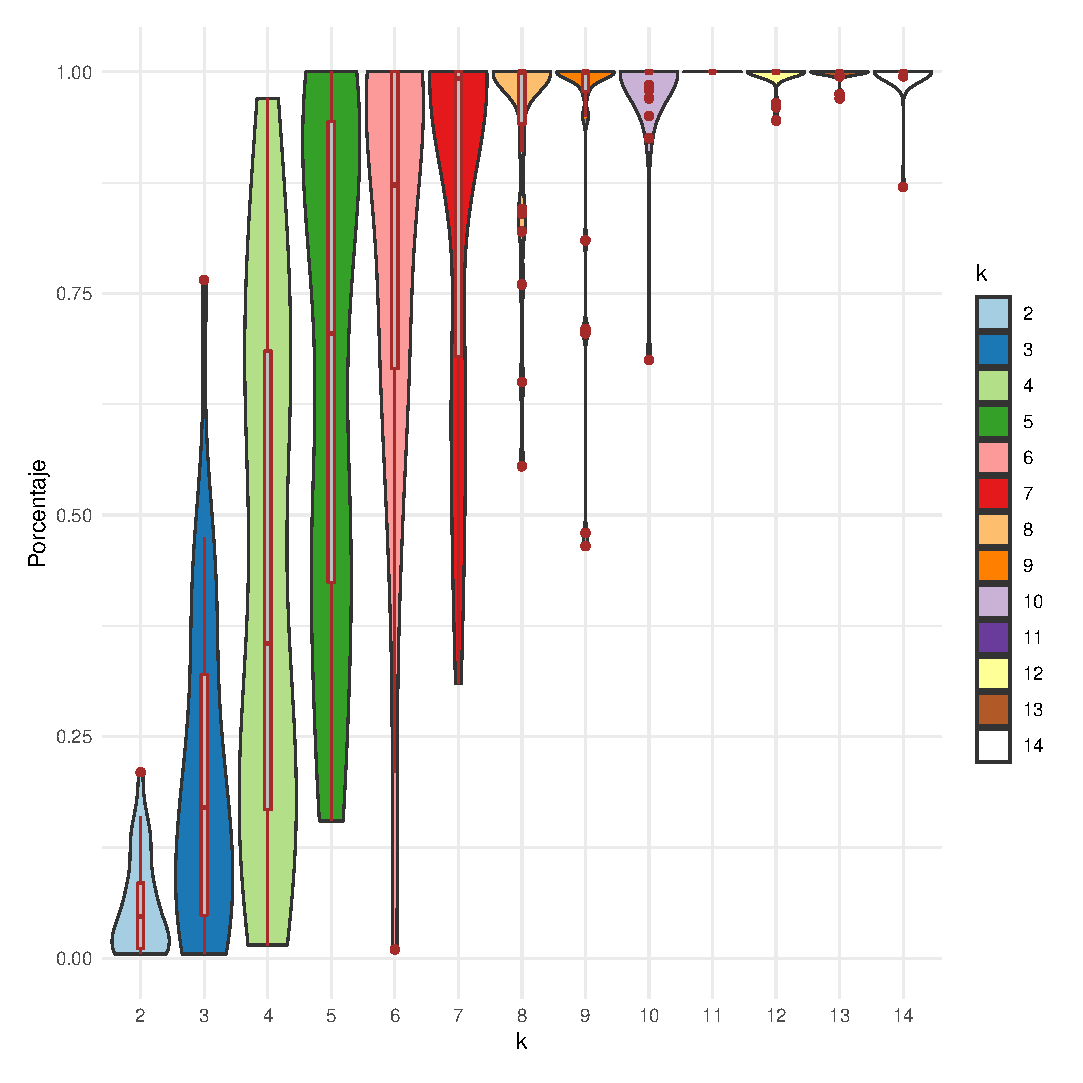
\includegraphics[width=85mm]{numdfunobjetiva.eps}
\caption{Porcentaje de soluciones}
\label{PS}
\end{figure}

Asimismo, se realizó una prueba \textit{Shapiro-Wilk} para verificar la probabilidad de una distribución normal; es una manera eficiente para determinar la normalidad de las variables. Por otro lado, se hizo una comprobación con \textit{kruskal.test} para evidenciar la existencia de alguna diferencia entre los niveles, además se ejecutó una prueba \textit{Pairwise Wilcox} para presentar que niveles son los causantes de estas diferencias.\\

\begin{lstlisting}[language=R]
a <- shapiro.test(dat$Porcentaje)
a$p.value
a$p.value < 0.05
b <- kruskal.test(dat$Porcentaje~dat$k)
b$p.value
b$p.value < 0.05
c <- pairwise.wilcox.test(dat$Porcentaje, dat$k, p.adjust.method = "none")
c$p.value
c$p.value < 0.05
\end{lstlisting}

Por consiguiente, se obtuvieron los resultados de \textit{Shapiro-Wilk test} del código anterior, en donde se puede notar una diferencia en el valor $p< 0.05$, lo cual nos dice que hay diferencias relevantes en las cantidades de funciones objetivo. Por otra parte el valor $p< 0.05$ verificado con el \textit{kruskal.test} nos muestra que solamente en algunos niveles las diferencias son despreciables. Por último con el \textit{Pairwise Wilcox test} se expone con un \textit{TRUE} a los niveles que presentan dichas diferencias.\\

\begin{lstlisting}[language=R]

a <- shapiro.test(dat$Porcentaje)
a$p.value
[1] 1.030554e-25
a$p.value < 0.05
[1] TRUE
b <- kruskal.test(dat$Porcentaje~dat$k)
b$p.value
[1] 7.036467e-50
b$p.value < 0.05
[1] TRUE

c <- pairwise.wilcox.test(dat$Porcentaje, dat$k, p.adjust.method = "none")
c$p.value  

      2    3    4     5     6    7     8     9    10    11    12    13 
3  TRUE   NA   NA    NA    NA   NA    NA    NA    NA    NA    NA    NA
4  TRUE TRUE   NA    NA    NA   NA    NA    NA    NA    NA    NA    NA
5  TRUE TRUE TRUE    NA    NA   NA    NA    NA    NA    NA    NA    NA
6  TRUE TRUE TRUE FALSE    NA   NA    NA    NA    NA    NA    NA    NA
7  TRUE TRUE TRUE FALSE FALSE   NA    NA    NA    NA    NA    NA    NA
8  TRUE TRUE TRUE  TRUE FALSE TRUE    NA    NA    NA    NA    NA    NA
9  TRUE TRUE TRUE  TRUE  TRUE TRUE FALSE    NA    NA    NA    NA    NA
10 TRUE TRUE TRUE  TRUE  TRUE TRUE  TRUE FALSE    NA    NA    NA    NA
11 TRUE TRUE TRUE  TRUE  TRUE TRUE  TRUE  TRUE  TRUE    NA    NA    NA
12 TRUE TRUE TRUE  TRUE  TRUE TRUE  TRUE FALSE FALSE  FALSE FALSE FALSE
13 TRUE TRUE TRUE  TRUE  TRUE TRUE  TRUE FALSE FALSE  FALSE FALSE    NA
14 TRUE TRUE TRUE  TRUE  TRUE TRUE  TRUE  TRUE  TRUE  FALSE FALSE FALSE

\end{lstlisting}

\subsection{Reto 1}

Para el primer reto se creó un código, de acuerdo al trabajo anteriormente reportado \cite{P11}. En el cual se seleccionó un subconjunto que permita observar el comportamiento del tamaño del porcentaje del frente de Pareto y este actué de modo diverso, ocasionando una agrupación en una sola zona, cercana a las soluciones.\\

\begin{lstlisting}[language=R]
cluster <- makeCluster(detectCores()- 1)
clusterExport(cluster, c("domin.by", "sign", "eval", "poli", "n", "pick.one"))

dat <- rbind(dat, c(k, replicas, sum(no.dom)/n))
    Select <- frente[c(round(runif(round(dim(frente)[1]/2), min = 1, max = dim(frente)[1]))),]
    Select1 <- data.frame()
    Select1 <- rbind(Select1, Select)

vec <- seq(1, k, by = 1)
    for (i in vec) {
      if((i+1) == is.element(i+1, vec)*(i+1)){
        png(paste("p11_frente", k, "_", replicas, "_", i, "-", i+1, ".png", sep=""))
        xt = paste("Objetivo ", i, " (", cual[minim[i] + 1], ")", sep = "")
        yt = paste("Objetivo ", i+1, " (", cual[minim[i+1] + 1], ")", sep = "")
        plot(val[,i], val[,i+1], xlab=xt, ylab=yt)
        points(frente[,i], frente[,i+1], col="green", pch=16, cex=1.5)
        points(Select1[,i], Select1[,i+1], col="red", pch=16, cex=1.5)
        graphics.off()
      }
    }
    data <- data.frame(pos=rep(0, n), dom=dominadores)
\end{lstlisting}

En la figura \ref{DV} se manifiesta un frente diversificado en atención a lo cual los puntos rojos son los puntos del frente de Pareto y los verdes al frente original.  Se puede notar que al aumentar los pasos en la ejecución del código los puntos rojos van disminuyendo, debido a la selección determinada en el código anterior.

\begin{figure}[H]
\centering
\subfigure[Paso 1]{\includegraphics[width=56mm]{./p11_frente2_2_1-2}}\vspace{1mm}
\subfigure[Paso 6]{\includegraphics[width=56mm]{./p11_frente2_6_1-2}}
\subfigure[Paso 9]{\includegraphics[width=56mm]{./p11_frente2_9_1-2}}
\caption{Divergencia de variables}\label{DV}
\end{figure}


\subsection{Reto 2}

En el segundo reto se realizo una combinación del código del algoritmo genético \cite{elisawebgen} con el proporcionado para esta práctica, para realizar una especie de selección natural que permita tener una mejor generación de la población inicial, como se muestra en las siguientes líneas de código.\\

\begin{lstlisting}[language=R]
conquered <- function(i){
  d <- logical()
  for (j in 1:n) {
    d <- c(d, domin.by(sign * val[i,], sign * val[j,], k))
  }
  return(d)
}

cluster <- makeCluster(detectCores() - 1)
clusterExport(cluster, "verify")
clusterExport(cluster, "eval")
clusterExport(cluster, "obj")
clusterExport(cluster, "sol")
clusterExport(cluster, "tc")
clusterExport(cluster, "k")
clusterExport(cluster, "n")

val <- parSapply(cluster, 1:n, verify)
val <- t(val)
stopCluster(cluster)

mejor1 <- which.max(sign[1] * val[,1])
mejor2 <- which.max(sign[2] * val[,2])
cual <- c("max", "min")
xl <- paste("Primer objetivo (", cual[minim[1] + 1], ")", sep="")
yl <- paste("Segundo objetivo (", cual[minim[2] + 1], ")", sep="")

no.dom <- logical()
conqueredres <- integer()

cluster <- makeCluster(detectCores() - 1) 
clusterExport(cluster, "conquered")
clusterExport(cluster, "domin.by")
clusterExport(cluster, "val")
clusterExport(cluster, "sign")
clusterExport(cluster, "k")
clusterExport(cluster, "n")

d <- parSapply(cluster, 1:n, conquered)
stopCluster(cluster)

for(x in 1:nrow(sol)){
    cuantos <- sum(d[,x])
    conqueredres <- c(conqueredres, cuantos)
    no.dom <- c(no.dom, cuantos == 0) 
    dom <- c(dom, cuantos != 0)
}
frente <- subset(val, no.dom) 

mutacion <- function(sol, vc) {
  pos <- sample(1:vc, 1)
  mut <- sol
  delta <- 0.1
  mut[pos] <- (sol[pos]) * delta
  return(mut)
}

muta <- function(i){
  if (runif(1) < pm) {
    return(mutacion(sol[i,], vc))
  }
  else{
    return(sol[i,])
  }
}

reproduccion <- function(x, y, vc) { 
  pos <- sample(2:(vc-1), 1)
  xy <- c(x[1:pos], y[(pos+1):vc])
  yx <- c(y[1:pos], x[(pos+1):vc])
  return(c(xy, yx))
}


cluster <- makeCluster(detectCores() - 1)

pm <- 0.05 
rep <- 50 
tmax <- 100 
for (iter in 1:tmax) { 

clusterExport(cluster, "pm")
  clusterExport(cluster, "vc")
  clusterExport(cluster, "sol")
  clusterExport(cluster, "mutacion")
  clusterExport(cluster, "muta")
  sol <- t(parSapply(cluster, 1:n,muta)) 

  for (i in 1:rep) { 
    padres <- sample(1:n, 2, replace=FALSE)
    hijos <- reproduccion(sol[padres[1],], sol[padres[2],], vc)
    sol <- rbind(sol, hijos[1:vc]) # primer hijo
    sol <- rbind(sol, hijos[(vc+1):(2*vc)]) # segundo hijo
  }
  val <- matrix(rep(NA, k * nrow(sol)), nrow=nrow(sol), ncol=k)
  clusterExport(cluster, "verify")
  clusterExport(cluster, "eval")
  clusterExport(cluster, "obj")
  clusterExport(cluster, "sol")
  clusterExport(cluster, "tc")
  clusterExport(cluster, "k")
  clusterExport(cluster, "n")
  val <- parSapply(cluster, 1:nrow(sol), verify)
  val <- t(val)
  no.dom <- logical()
  dom <- logical()
  conqueredres <- integer()
  clusterExport(cluster, "conquered")
  clusterExport(cluster, "domin.by")
  clusterExport(cluster, "val")
  clusterExport(cluster, "sign")
  clusterExport(cluster, "k")
  clusterExport(cluster, "n")
  
  d <- parSapply(cluster, 1:nrow(sol), conquered)
  for(x in 1:nrow(sol)){
    cuantos <- sum(d[,x])
    conqueredres <- c(conqueredres, cuantos)
    no.dom <- c(no.dom, cuantos == 0) 
    dom <- c(dom, cuantos != 0)
  }
  frente_sol <- subset(sol, no.dom) 
  dominadas <- subset(sol, dom)
  frente <- subset(val, no.dom) 
  domi <- order(conqueredres)
  domi <- domi[1:n]
  
  sol <- sol[domi,]
  val <- val[domi,]
  digitos <- floor(log(tmax, 10)) + 1
  tl <- paste0(iter, "", sep="")
  while (nchar(tl) < digitos) {
    tl <- paste("0", tl, sep="")
  }

 if(nrow(frente) == n)
  {
    break;
  }
}
stopCluster(cluster)
system("convert -delay 50 -size 300x300 Genetico*.png -loop 0 Gen.gif")
\end{lstlisting}

Fueron seleccionadas cinco representaciones gráficas significativas del cambio, que conforman a la figura \ref{DAGen}, en la cual se muestra la distribución ocasionada por el algoritmo genético, que en virtud de ello el frente tiene cambios relevantes en las primeras generaciones, después de la octava generación las soluciones se van homogeneizando ligeramente.

\begin{figure}[H]
\centering
\subfigure[Generación 1]{\includegraphics[width=65mm]{./Genetico001}}\vspace{0mm}
\subfigure[Generación  3]{\includegraphics[width=65mm]{./Genetico003}}
\subfigure[Generación  5]{\includegraphics[width=65mm]{./Genetico005}}
\subfigure[Generación  8]{\includegraphics[width=65mm]{./Genetico008}}
\subfigure[Generación  9]{\includegraphics[width=65mm]{./Genetico009}}
\subfigure[Generación 10]{\includegraphics[width=65mm]{./Genetico010}}
\caption{Distribución de algoritmo genético}\label{DAGen}
\end{figure}

\bibliographystyle{plainnat}

\bibliography{BiblioHWP11}

\end{document}